\documentclass[
      10pt,
          aspectratio = 169,
  ]{beamer}

\usepackage[english]{babel}
\usepackage[T1]{fontenc}
\usepackage{amsmath, amssymb}
\usepackage{animate}
\usepackage{xcolor}
\usepackage{hyperref}
\usepackage{verbatim}
\usepackage{graphicx}
\usepackage{etoolbox}

% programming
\newcommand{\code}[1]{\texttt{#1}}
\newcommand{\class}[1]{`\code{#1}'}
\newcommand{\fct}[1]{\code{#1()}}
\newcommand{\pkg}[1]{\{\code{#1}\}}
\newcommand{\lang}[1]{\code{#1}}

% math
\newcommand{\R}{\mathbb{R}}

% statistic
\newcommand{\var}{\operatorname{Var}}
\newcommand{\E}{\operatorname{E}}
\newcommand{\cov}{\operatorname{Cov}}
\newcommand{\sd}{\operatorname{sd}}
\newcommand{\se}{\operatorname{se}}
\newcommand{\mean}{\operatorname{mean}}
\newcommand{\Prob}{\operatorname{Prob}}


  \usepackage[no-math]{fontspec}
  \setmainfont[
      Path            = ./theme/,
      Extension       = .otf,
      Ligatures       = TeX,
      UprightFont     = *-Regular,
      ItalicFont      = *-RegularItalic,
      BoldFont        = *-Bold,
      BoldItalicFont  = *-BoldItalic
  ]{Lelo}

  \usepackage{theme/eco_bielefeld}

  \usepackage{emoji}

\providecommand{\tightlist}{%
  \setlength{\itemsep}{0pt}\setlength{\parskip}{0pt}}

  \title{Title}

\makeatletter
\providecommand{\subtitle}[1]{% add subtitle to \maketitle
  \apptocmd{\@title}{\par {\large #1 \par}}{}{}
}
\makeatother
\subtitle{Subtitle}

\author[Presenter]{Presenter}

\date{2023-07-28}

  \institute{Institute}

\AtBeginSection[]
{
    \begin{frame}
        \frametitle{Outline}
        \tableofcontents[currentsection]
    \end{frame}
}

\usepackage{fontawesome}

\begin{document}

  \begin{frame}[plain]{}
    \titlepage
  \end{frame}

  \begin{frame}
    \frametitle{Outline}
    \tableofcontents
  \end{frame}

\hypertarget{section-1}{%
\section{Section 1}\label{section-1}}

\begin{frame}[fragile]{LaTeX Engine}
\protect\hypertarget{latex-engine}{}
\begin{itemize}
\tightlist
\item
  This template uses the \href{https://camelot-typefaces.com/lelo}{Lelo
  font}.
\item
  The font is set via \texttt{\textbackslash{}usepackage\{fontspec\}},
  which requires XeLaTeX or LuaLaTeX.
\item
\item
  When compiling this template, make sure that either XeLaTeX or
  LuaLaTeX is the selected LaTeX engine.
\end{itemize}
\end{frame}

\begin{frame}{Subsection 1.2}
\protect\hypertarget{subsection-1.2}{}
\begin{itemize}
\tightlist
\item
  Eat eggs
\item
  Drink coffee
\end{itemize}
\end{frame}

\hypertarget{section-2}{%
\section{Section 2}\label{section-2}}

\begin{frame}{Subsection 2.1}
\protect\hypertarget{subsection-2.1}{}
\begin{itemize}
\tightlist
\item
  Eat spaghetti
\item
  Drink wine
\end{itemize}
\end{frame}

\begin{frame}
\begin{figure}
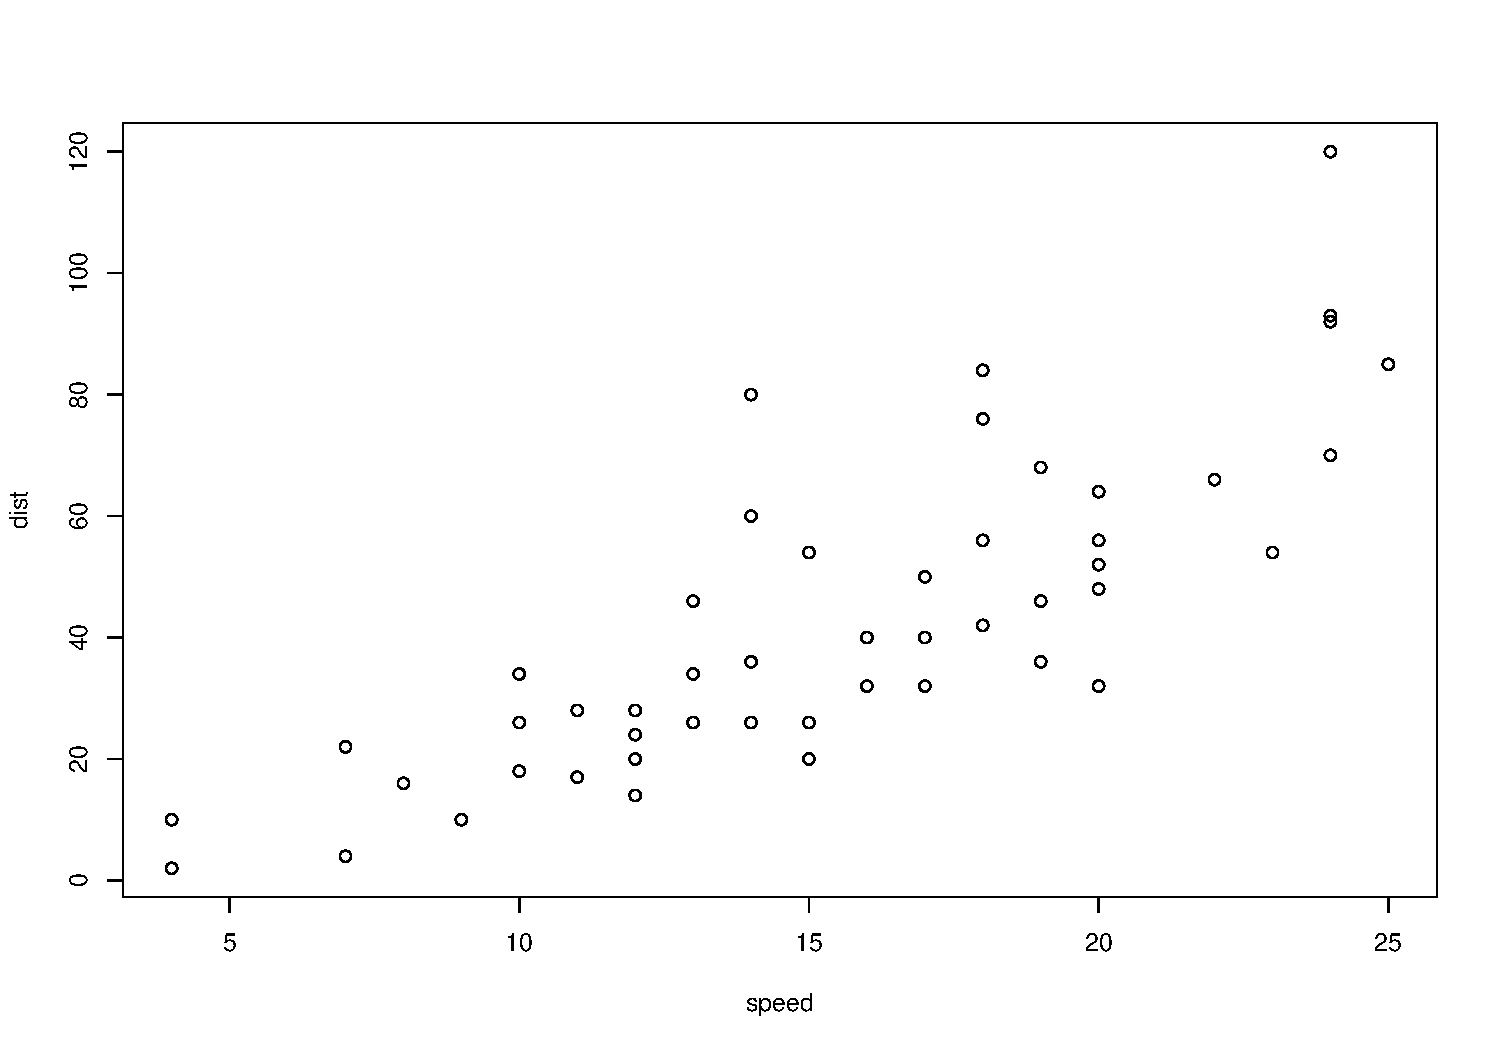
\includegraphics[height=0.7\textheight]{figures/cars-1} \caption{A scatterplot.}\label{fig:cars}
\end{figure}
\end{frame}

\begin{frame}{Subsection 2.2}
\protect\hypertarget{subsection-2.2}{}
\begin{itemize}
\tightlist
\item
  Get in bed
\item
  Count sheep
\end{itemize}
\end{frame}

  \begin{frame}{}
      \vspace{0.5cm}
      \begin{center}
          {\Large Thanks for your attention!}
      \end{center}
      \vfill
      \begin{itemize}
        \item[\faEnvelope] \href{mailto:someone@example.com}{someone@example.com} \\
        \item[\faLaptop] \href{https://example.org/}{https://example.org/}
      \end{itemize}
  \end{frame}

\end{document}